\part*{}

\chapter{Schlussbetrachtungen} % (fold)
\label{cha:schlussbetrachtungen}

\begin{figure}[htbp]
	\centering
		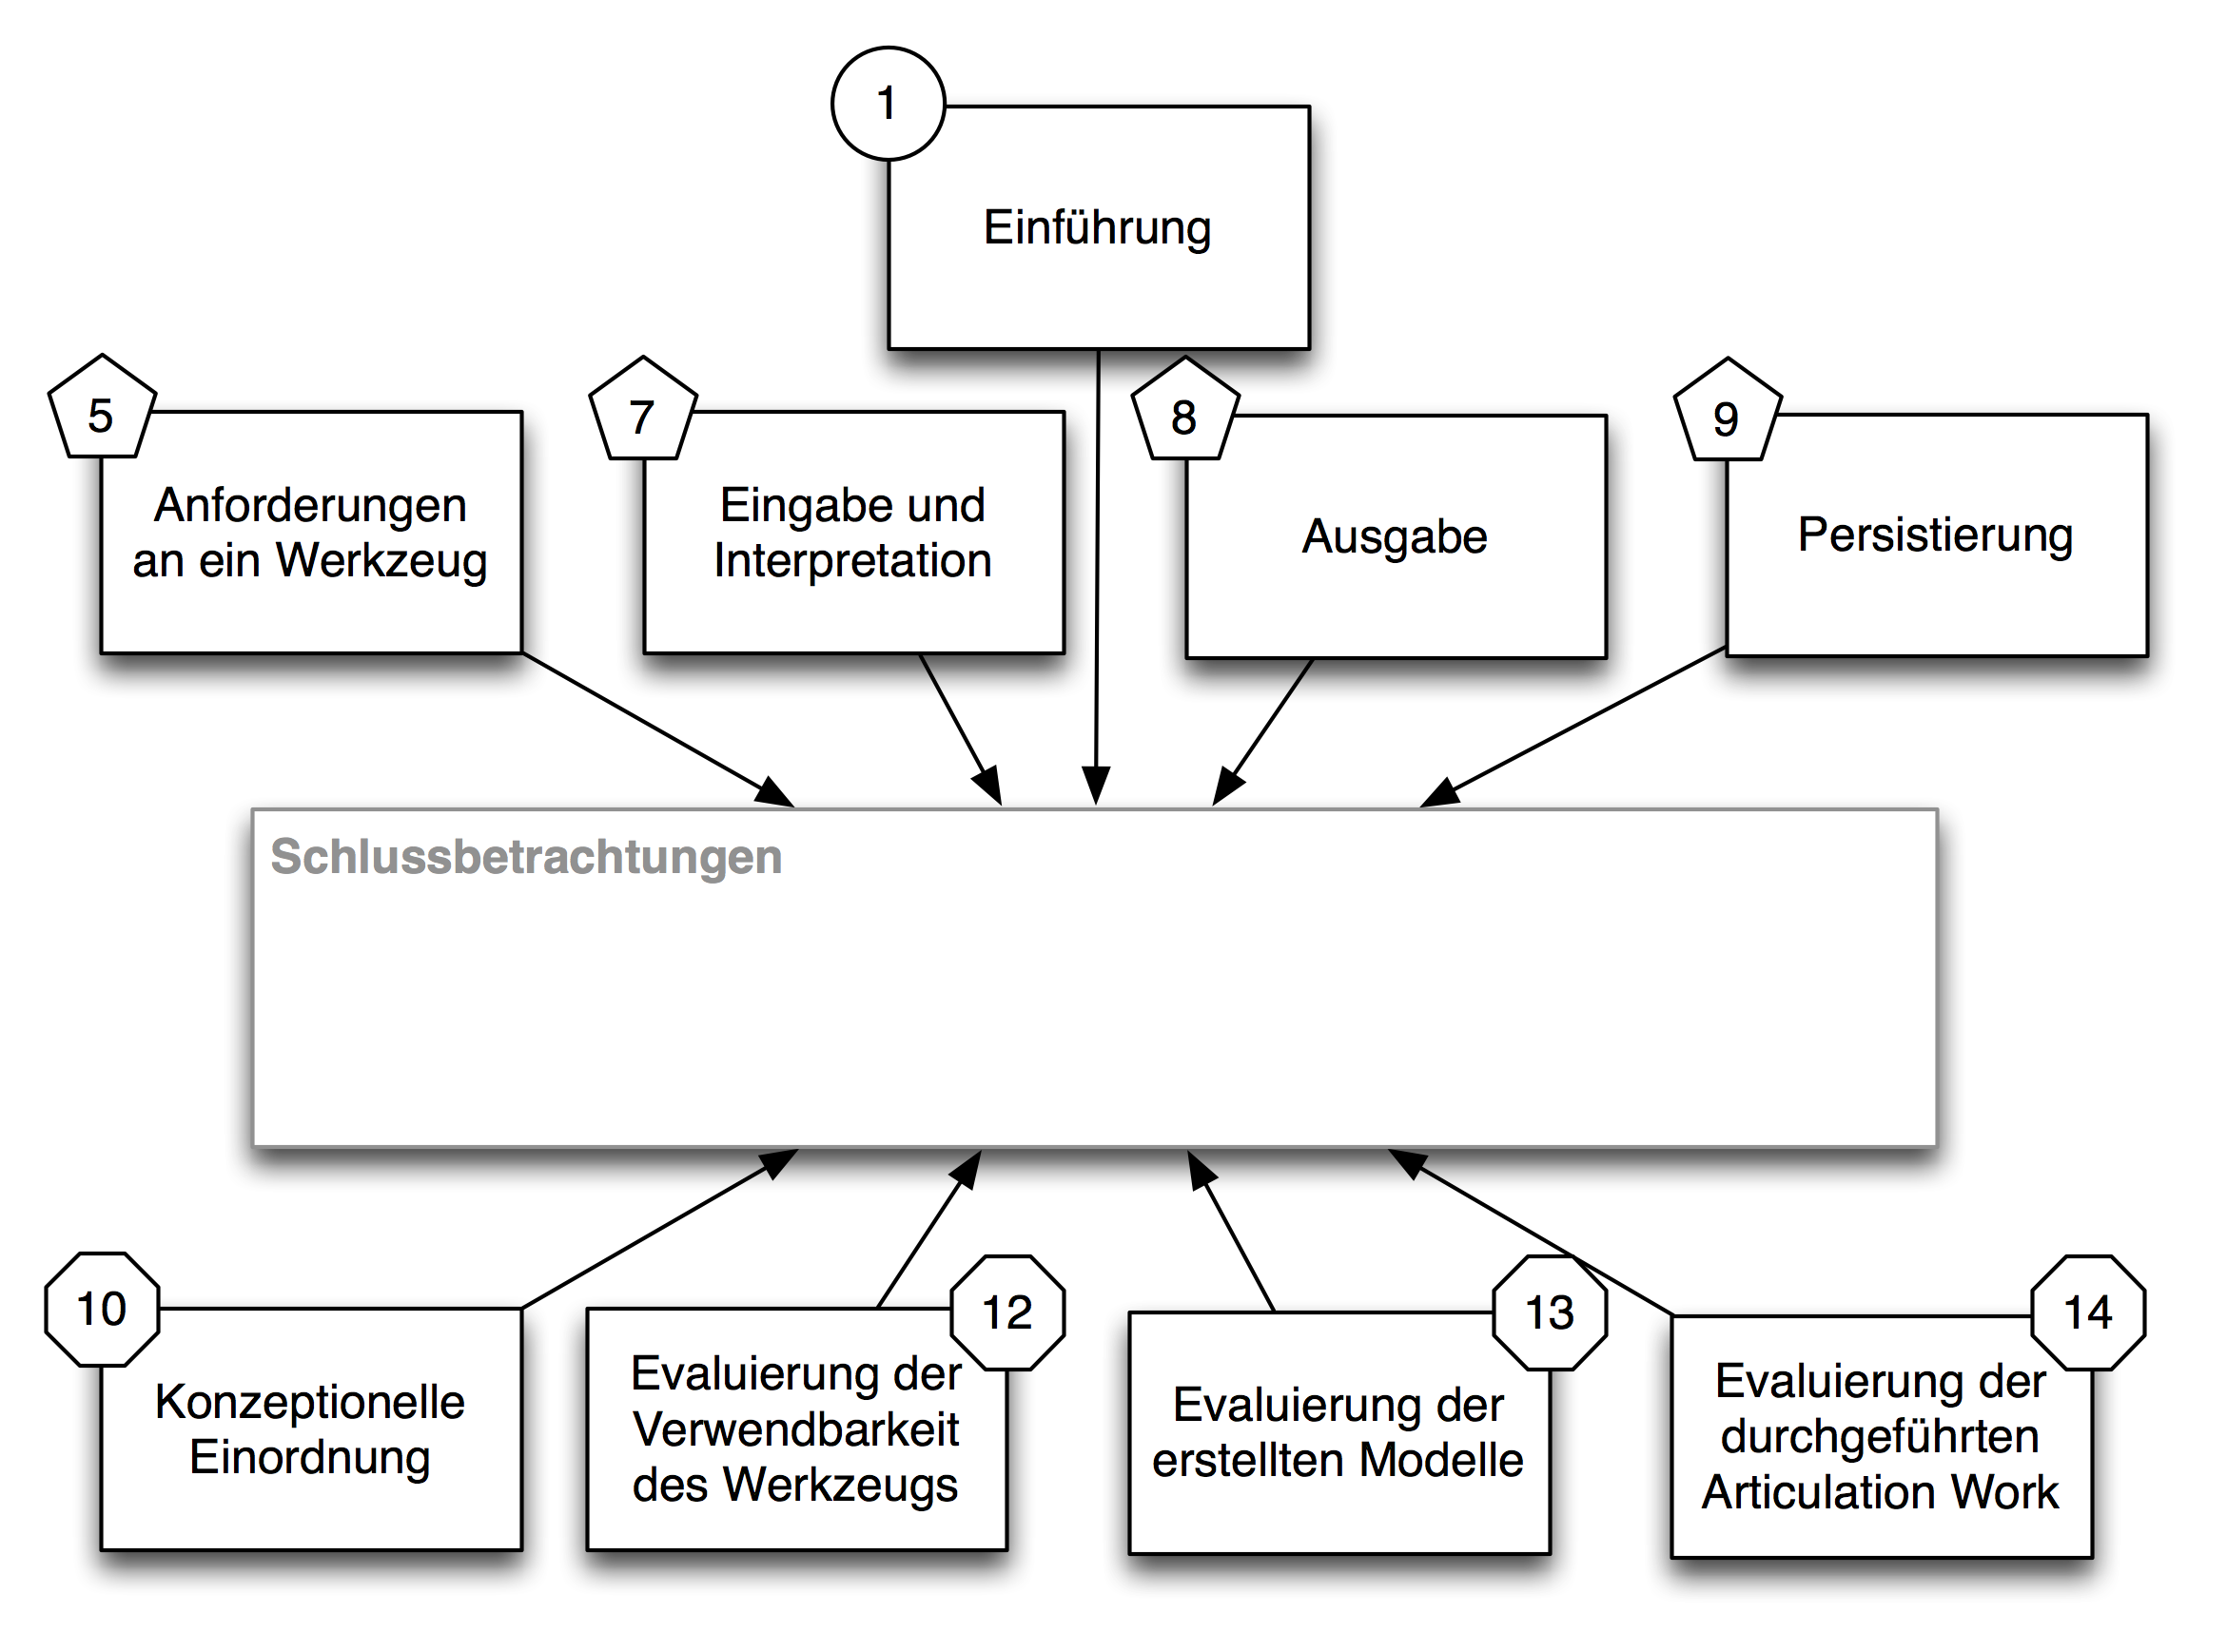
\includegraphics[scale=0.7]{img/Kontextgrafiken/k15.png}
	\caption{Kapitel „Schussbetrachtungen“ im Gesamtzusammenhang}
	\label{fig:img_Kontextgrafiken_k15}
\end{figure}

\section{Überblick über den Gesamtzusammenhang} % (fold)
\label{sec:überblick_über_den_gesamtzusammenhang}

\begin{figure}[htbp]
	\centering
		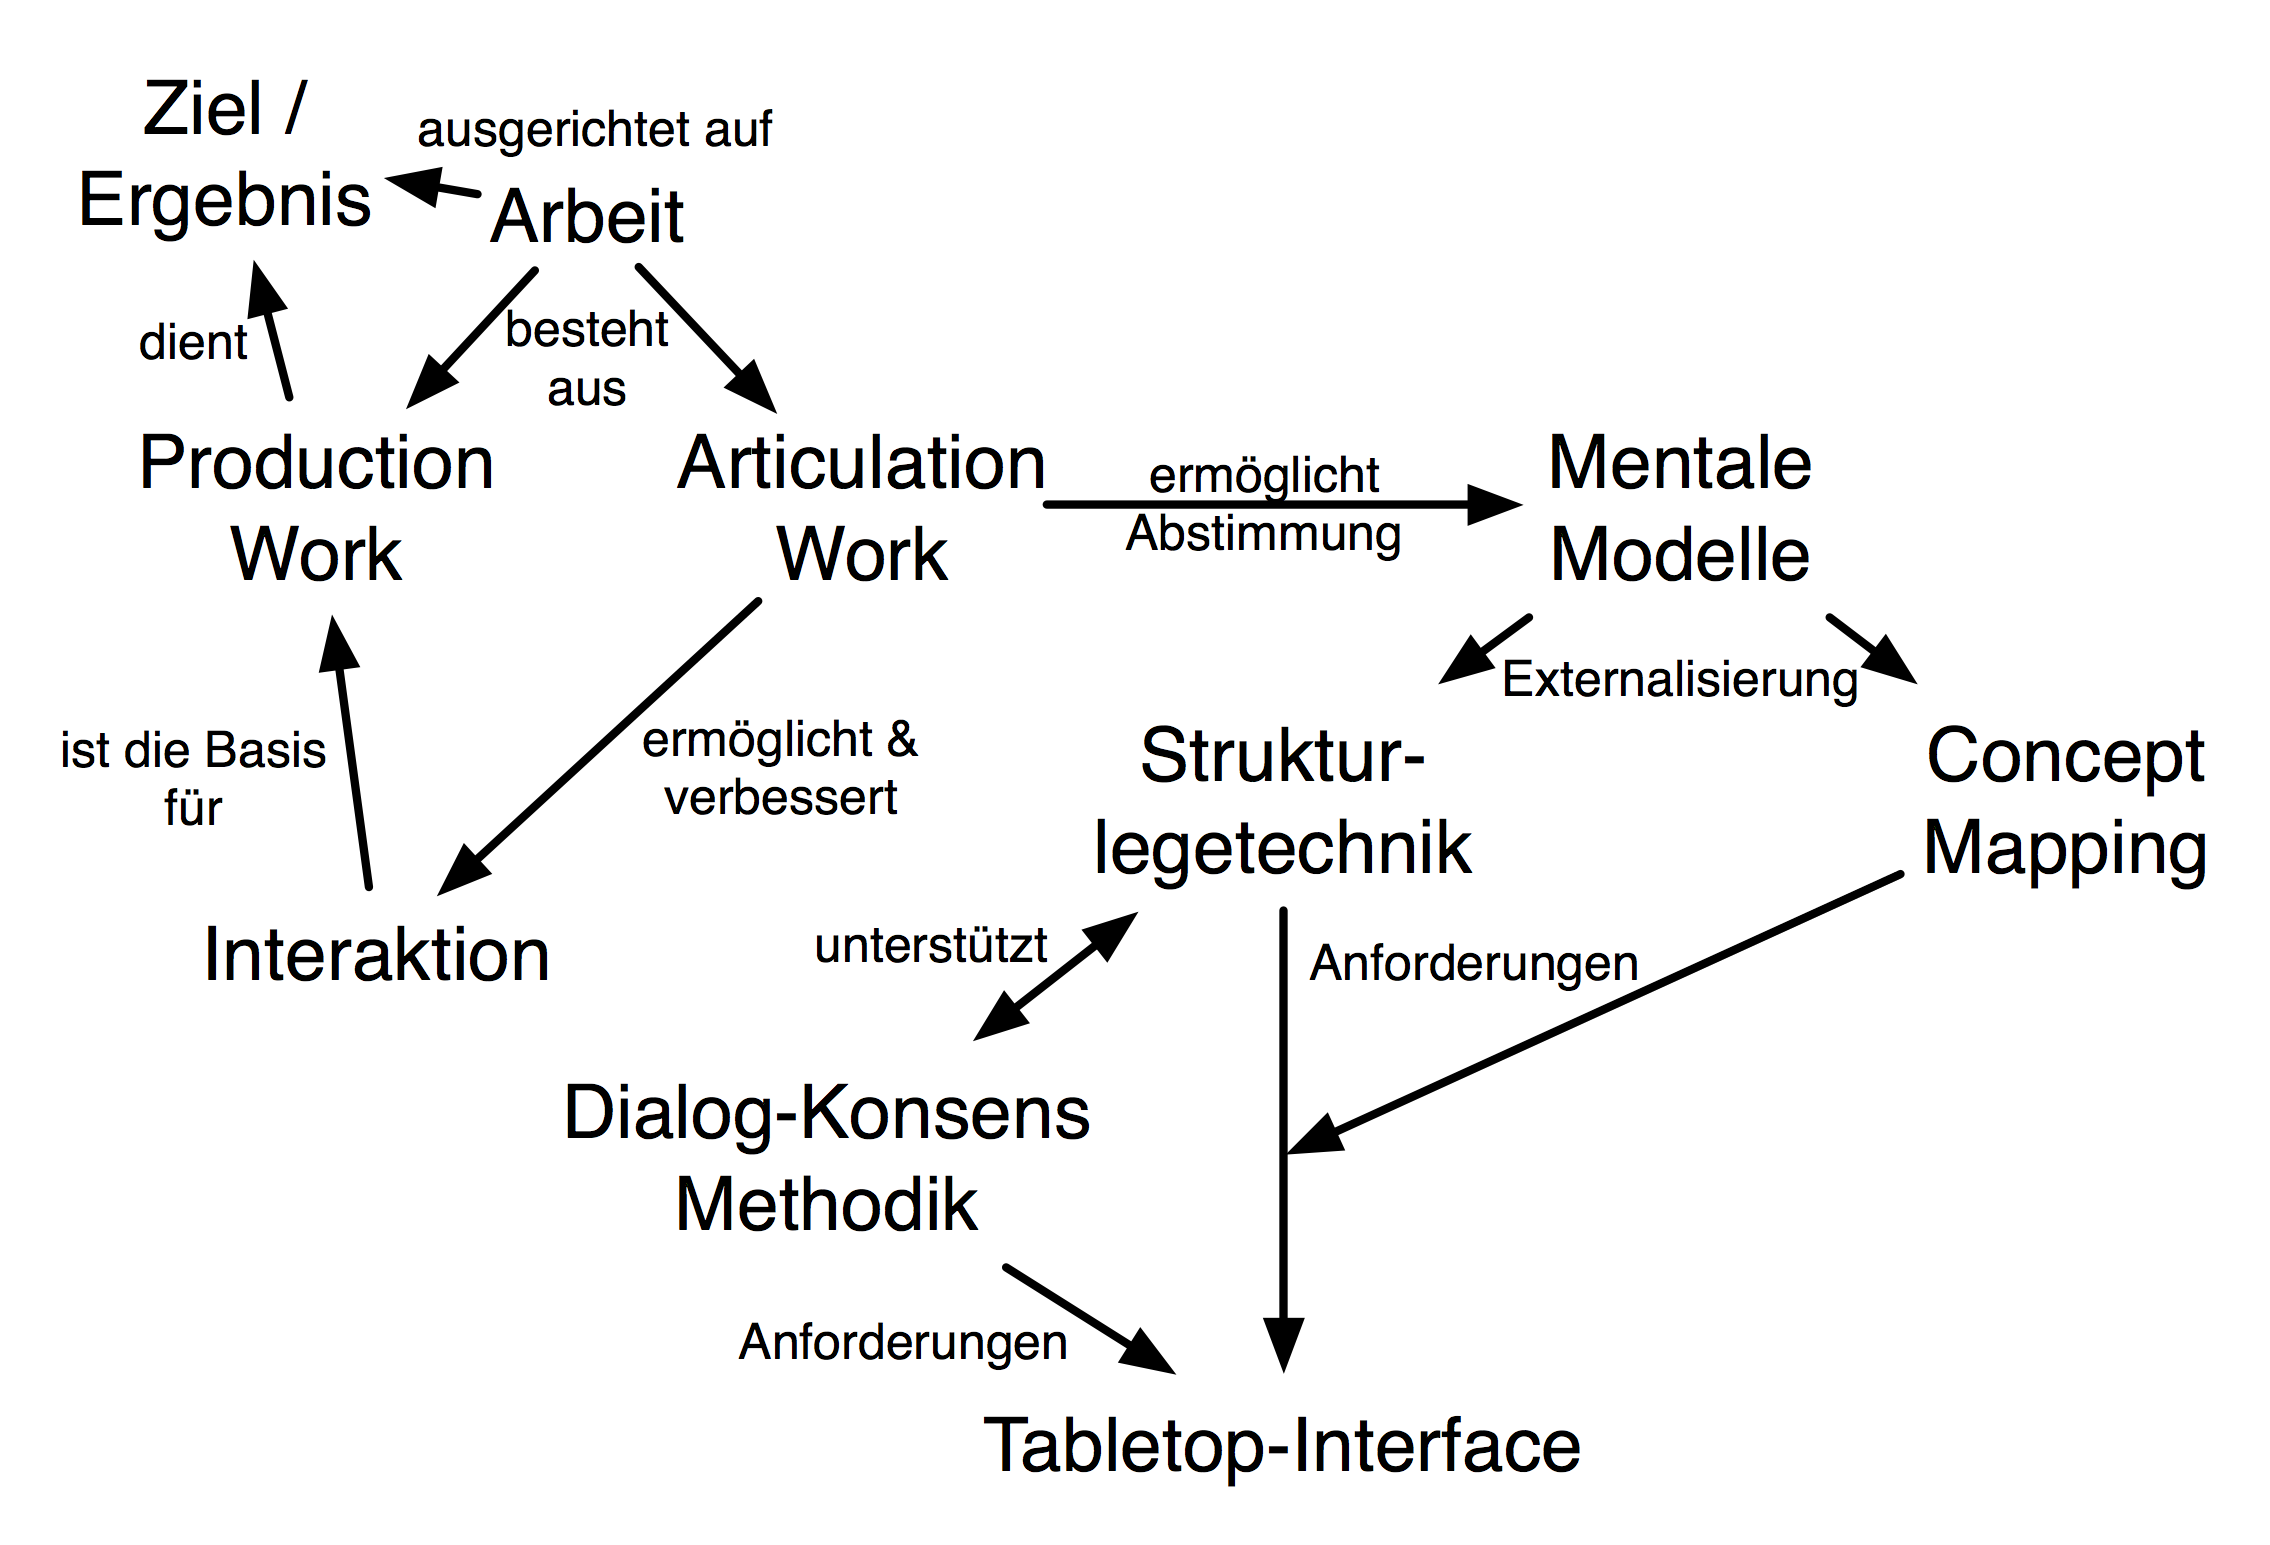
\includegraphics[width=10cm]{img/Schlussbetrachtungen/ArbeitInteraktionMentaleModelleTabletop.png}
	\caption{Gesamtzusammenhang der in dieser Arbeit verwendeten Konzepte}
	\label{fig:img_Schlussbetrachtungen_ArbeitInteraktionMentaleModelleTabletop}
\end{figure}

evtl. noch zweite Grafik, die die Kapitel der Arbeit in diese Struktur einordnet.

% section überblick_über_den_gesamtzusammenhang (end)

\section{Zusammenfassung der Evaluierung}

In diesem Abschnitt wird die in den Kapiteln \ref{cha:eval_ueberblick}, \ref{cha:eval_werkzeug}, \ref{cha:eval_modell} und \ref{cha:eval_aw} beschriebene empirische Untersuchung zusammengefasst und den Ergebnissen der konzeptuellen Einordnung in Kapitel \ref{cha:konzeptionelle_evaluierung} gegenübergestellt.

\subsection{Empirische Untersuchung}

In der empirischen Untersuchung waren folgende in Kapitel \ref{cha:eval_ueberblick} formulierte Untersuchungsfragen zu beantworten:

\begin{itemize}
 \item Sind das Werkzeug und dessen Komponenten verständlich und wie intendiert einsetzbar? (Aspekt: Werkzeug)
 \item Erlauben Werkzeug und Methode die Abbildung semantisch offener diagrammatischer Modelle? (Aspekt: Modell)
 \item Unterstützen Werkzeug und Methode Articulation Work? (Aspekt: Articulation Work)
\end{itemize}

\subsection{Gegenüberstellung der empirischen und konzeptuellen Untersuchung}

noch offen

\section{Erfüllung der Anforderungen an das Werkzeug}

In diesem Abschnitt werden die in Kapitel \ref{cha:anforderungen} formulierten Anforderungen an das Werkzeug hinsichtlich ihrer Erfüllung betrachtet. Die Beurteilung der Erfüllung erfolgt anhand der empirischen Ergebnisse, die in den Kapiteln \ref{cha:eval_werkzeug}, \ref{cha:eval_modell} und \ref{cha:eval_aw} beschrieben wurden.

Anforderung \ref{anf:physische_abbildung_legen_beliebiger_diagrammatischer_modelle} (Physische Abbildung beliebiger diagrammatischer Modelle) wurde in den Hypothesen \ref{hyp:diagmodelle}, \ref{hyp:behinderung} und \ref{hyp:gewöhnung} untersucht.

Anforderung \ref{anf:unterstützung_der_iterativen_aushandlung_des_modells} (Unterstützung der iterativen Aushandlung des Modells) wurde in der Hypothese \ref{hyp:abstimmung} untersucht.

Anforderung \ref{anf:ermöglichung_experimenteller_veränderungen_am_modell} (Ermöglichung experimenteller Veränderungen am Modell) wurde in der Hypothese \ref{hyp:wiederherstellung} untersucht.

Anforderung \ref{anf:nicht_vorgegebene_semantik_der_modellierungselemente} (Nicht vorgegebene Semantik der Modellierungselemente) wurde in den Hypothesen \ref{hyp:kontexte} und \ref{hyp:keine_einschränkung} untersucht.

Anforderung \ref{anf:verknüpfung_mit_digitalen_ressourcen} (Verknüpfung mit digitalen Ressourcen) wurde im Rahmen der empirischen Untersuchung nicht berücksichtigt.

Anforderung \ref{anf:bearbeitung_von_beliebig_komplexen_modellen} (Bearbeitung von beliebig umfangreicher Modellen) wurde in der Hypothese \ref{hyp:beliebige_komplexität} untersucht.

Anforderung \ref{anf:kollaborative_und_unmittelbare_manipulierbarkeit_des_modells} (Kooperative und unmittelbare Manipulierbarkeit des Modells) wurde in den Hypothesen \ref{hyp:kollaborativ} und \ref{hyp:stärkere_kooperation} untersucht.

Anforderung \ref{anf:persistente_ablage_des_modells_möglichkeit_zur_rekonstruktion} (Persistente Ablage des Modells und Möglichkeit zur Rekonstruktion) wurde in der Hypothese \ref{hyp:historie} untersucht.

Zusammenfassend ergibt sich hinsichtlich der Erfüllung der Anforderungen folgende Übersicht. In ihr sind die Anforderungen jenen Kapiteln und Abschnitten des Implementierungsteils (\emph{Impl.}) zugewiesen, in denen ihre technische Umsetzung beschrieben wird, sowie den Hypothesen (\emph{Hyp.}) zugeordnet, in denen die tatsächliche Überprüfung der Erfüllung durchgeführt wird.

\begin{center}
\begin{tabular}{| c | p{5cm} | p{1cm} | c | p{4cm} |} 
  \hline
  & Anforderung & Impl. & Hyp. & Beurteilung \\ \hline \hline
  \ref{anf:physische_abbildung_legen_beliebiger_diagrammatischer_modelle} & Physische Abbildung beliebiger diagrammatischer Modelle &  \ref{sub:erkennen_von_verbindungen}, \ref{sub:benennung_von_modellelementen}, \ref{sub:ausgabe_von_information_zum_modell} & \ref{hyp:diagmodelle}, \ref{hyp:behinderung}, \ref{hyp:gewöhnung} & technisch möglich, empirisch bestätigt \\ \hline
  \ref{anf:unterstützung_der_iterativen_aushandlung_des_modells} & Unterstützung der iterativen Aushandlung des Modells & \ref{ssub:zustands_und_ereignismeldungen} & \ref{hyp:abstimmung} & technisch möglich, empirisch bestätigt \\ \hline
  \ref{anf:ermöglichung_experimenteller_veränderungen_am_modell} & Ermöglichung experimenteller Veränderungen am Modell & \ref{sub:tracking_des_modellzustandes}, \ref{ssub:wiederherstellungsunterstützung} & \ref{hyp:wiederherstellung} & technisch möglich, empirisch nicht bestätigt \\ \hline \hline
  \ref{anf:nicht_vorgegebene_semantik_der_modellierungselemente} & Nicht vorgegebene Semantik der Modellierungselemente & \ref{sub:festlegung_der_bedeutung_von_modellelementen}, \ref{sub:abbildung_des_metamodells} & \ref{hyp:kontexte}, \ref{hyp:keine_einschränkung} & technisch möglich, empirisch bestätigt \\ \hline
  \ref{anf:verknüpfung_mit_digitalen_ressourcen} & Verknüpfung mit digitalen Ressourcen & \ref{sub:erkennung_von_geöffneten_tokens}, \ref{sub:ausgabe_von_information_zum_modell} & --- & technisch möglich, empirisch nicht geprüft \\ \hline
  \ref{anf:bearbeitung_von_beliebig_komplexen_modellen} & Bearbeitung von beliebig umfangreicher Modellen & \ref{sub:erkennung_von_geöffneten_tokens} & \ref{hyp:beliebige_komplexität} & technisch möglich, empirisch nicht bestätigt \\ \hline \hline
  \ref{anf:kollaborative_und_unmittelbare_manipulierbarkeit_des_modells} & Kooperative und unmittelbare Manipulierbarkeit des Modells & \ref{sub:verteilung_des_modellzustandes}, \ref{sub:einsatz_von_jhotdraw} & \ref{hyp:kollaborativ}, \ref{hyp:stärkere_kooperation} & technisch möglich, empirisch bestätigt \\ \hline
  \ref{anf:persistente_ablage_des_modells_möglichkeit_zur_rekonstruktion} & Persistente Ablage des Modells und Möglichkeit zur Rekonstruktion & \ref{sub:tracking_des_modellzustandes}, \ref{ssub:abruf_der_modellierungshistorie}, \ref{sub:grundlegende_abbildung} & \ref{hyp:historie} & technisch möglich, empirisch bestätigt \\ \hline 
\end{tabular}

\end{center}


\section{Bewertung hinsichtlich der globalen Zielsetzung}

In Kapitel \ref{cha:einführung} wurde die globale Zielsetzung wie folgt formuliert:

\fbox{\parbox{13cm}{\textbf{In der vorliegenden Arbeit sind die methodischen und technischen Möglichkeiten zur Ermöglichung und Unterstützung von expliziter Articulation Work zu ergründen, die gewonnenen Erkenntnissen in einem Werkzeug umzusetzen und dessen Auswirkungen auf die Interaktion zur Verbesserung der Production Work zu bewerten.}}}

Diese Zielsetzung wurde in drei Forschungsfragen detailliert:
\begin{enumerate}
	\item Wie kann explizite Articulation Work ermöglicht und unterstützt werden?
	\item Was muss ein Werkzeug zur Unterstützung von expliziter Articulation Work leisten?
	\item Inwiefern unterstützt das entwickelte Werkzeug die Durchführung von Articulation Work?
\end{enumerate}

\section{Offene Aspekte und Entwicklungspotential}

noch offen

\section{Schluss}

hier rein: Schlussresümee

Hypothesen zeigen: Geeignet für Articulation Work, eher nicht geeignet für detaillierte Modellbildungen, technisch keine Probleme mehr.

Schlussfolgerung: Werkzeug unterstützt den Prozess der kommunikativen Abstimmung von mentalen Modellen, nicht aber die vollständige Externalisierung derselben.

% \section{Anwendungsszenarien} % (fold)
% \label{sec:anwendungsszenarien}
% 
% \subsection{Problembeschreibung und Arbeitsabstimmung}
% 
% Einzel- oder Gruppensessions. 
% 
% Aufgabenstellung: meist aus Arbeitsabläufen der beteiligten Personen
% 
% Merkmal: Tisch ist Mittel zum Zweck, gelegtes Modell fungiert als Diskussionsgrundlage. Modell ist statisch, wird einmal gelegt und nicht mehr verändert. Eher kompakte Modelle, die den Kontext eines Problems beschreiben. Die eigentliche Problematik ist selten explizit im Modell dargestellt.
% 
% Anwendungsbeispiele: Block 1, Block 2, Block 4 (Session 1-3).
% 
% Vorteile:
% 
% \subsection{Concept Mapping}
% 
% Einzel- oder Gruppensessions. 
% 
% Aufgabenstellung: zur Erhebung bzw. Überprüfung von domänenspezifischen (Struktur-)Wissen
% 
% Merkmal: Tisch 
% 
% Anwendungsbeispiele: Block 3, Block 5
% 
% \subsection{Strukturaufstellung und Manipulation}
% 
% Anwendungsbeispiele: Block 4 (Session 4).
% 
% AUfgabenstellung: Erhebung und Reflexion der Strukturen in denen Arbeitsabläufe situiert sind (Abteilungen, Personen, Kommunikationskanäle).
% 
% Merkmal: Modelle sind nicht statisch - werden nach der Erstellung zwar meist nicht erweitert aber in ihrer Struktur verändert (räumliche Relation der Knoten zueinander). 
% 
% % chapter schlussbetrachtungen (end)